
\chapter{Colas}

\label{Cola} \index{cola} \index{TAD!Cola} \index{cola de prioridad}
\index{TAD!cola de prioridad} \index{PEPS} \index{política para meter}
\index{cola de prioridad}

Este capítulo presenta dos TADs: la cola y la cola de prioridad. En
la vida real una \textbf{Cola} es una línea de clientes esperando
por algún servicio. En la mayoría de los casos, el primer cliente
en la línea es el próximo en ser atendido. Sin embargo, hay excepciones.
En los aeropuertos, los clientes cuyos vuelos están próximos a partir
se atienden, sin importar su posición en la cola. En los supermercados,
un cliente cortés puede dejar pasar a alguien que va a pagar unos
pocos víveres.

La regla que dictamina quién se atiende a continuación se denomina
\textbf{política de atención}. La más sencilla se denomina \textbf{PEPS},
por la frase ``Primero que Entra - Primero que Sale''. La política
más general es la que implementa una \textbf{cola de prioridad}, en
la que cada cliente tiene asignada una prioridad y siempre se atiende
el cliente con la prioridad más alta, sin importar el orden de llegada.
Es la política más general en el sentido de que la prioridad puede
asignarse bajo cualquier criterio: la hora de partida de un vuelo,
cuántos víveres se van a pagar, o qué tan importante es el cliente.
No todas las políticas de atención son ``justas,'' pero la justicia
está definida por el que presta el servicio.

El TAD Cola y la cola de prioridad TAD tienen el mismo conjunto de
operaciones. La diferencia está en la semántica de ellas: una cola
utiliza la política PEPS y una cola de prioridad usa la política de
prioridad.

\adjustpage{1}

\section{El TAD Cola}

\index{TAD!Cola} \index{Cola TAD} \index{implementación!Cola}
\index{Cola!implementación con lista}

El TAD Cola se define por la siguiente interfaz:
\begin{description}
\item [{texttt{\_\_init\_\_}:}] inicializa una Cola vacía.
\item [{texttt{meter}:}] agrega un nuevo objeto a la cola.
\item [{texttt{sacar}:}] elimina y retorna un objeto de la Cola. Entre
todos los que están dentro de la cola, el objeto retornado fue el
primero en agregarse
\item [{texttt{estaVacia}:}] revisa si la cola está vacía.
\end{description}

\section{Cola enlazada}

\index{Cola enlazada} \index{Cola!implementación enlazada}

Esta primera implementación del TAD Cola se denomina \textbf{Cola
enlazada} porque está compuesta de objetos \texttt{Nodo} enlazados.
Aquí está la definición:

\beforeverb 
\begin{pythoncode}
class Cola:
  def __init__(self):
    self.numElementos = 0
    self.primero = None

  def estaVacia(self):
    return (self.numElementos == 0)

  def meter(self, carga):
    nodo = Nodo(carga)
    nodo.siguiente = None
    if self.primero == None:
      # si esta vacia este nodo sera el primero
      self.primero = nodo
    else:
      # encontrar el ultimo nodo
      ultimo = self.primero
      while ultimo.siguiente: ultimo = ultimo.siguiente
      # pegar el nuevo
      ultimo.siguiente = nodo
    self.numElementos = self.numElementos + 1

  def sacar(self):
    carga = self.primero.carga
    self.primero = self.primero.siguiente
    self.numElementos = self.numElementos - 1
    return carga
\end{pythoncode}
\afterverb El método \texttt{estaVacia} es idéntico al de la \texttt{ListaEnlazada},
\texttt{sacar} es quitar el enlace del primer nodo. El método \texttt{meter}
es un poco más largo.

Si la cola está vacía, le asignamos a \texttt{primero} el nuevo nodo.

Si tiene elementos, recorremos la lista hasta el último nodo y pegamos
el nuevo nodo al final. Podemos detectar si hemos llegado al final
de la lista porque el atributo \texttt{siguiente} tiene el valor \texttt{None}.

Hay dos invariantes que un objeto \texttt{Cola} bien formado debe
cumplir. El valor de \texttt{numElementos} debe ser el número de nodos
en la Cola, y el último nodo debe tener en \texttt{siguiente} el valor
\texttt{None}. Verifique que este método satisfaga los dos invariantes.

\section{Desempeño}

\index{desempeño}

Usualmente, cuando llamamos un método, no nos interesan los detalles
de la implementación. Sin embargo, hay un ``detalle'' que quisiéramos
saber —el desempeño del nuevo método. ¿Cuánto tarda en ejecutarse
y cómo cambia el tiempo de ejecución a medida que el número de objetos
en la Cola crece?

Primero observemos al método \texttt{sacar}.

No hay ciclos ni llamados a funciones, así que el tiempo de ejecución
de este método es el mismo cada vez que se ejecuta. Los métodos de
este tipo se denominan operaciones de \textbf{tiempo constante}. De
hecho, el método puede ser mas rápido cuando la lista está vacía ya
que no entra al cuerpo del condicional, pero esta diferencia no es
significativa.

\index{tiempo constante}

El desempeño de \texttt{meter} es muy diferente. En el caso general,
tenemos que recorrer la lista para encontrar el último elemento.

Este recorrido toma un tiempo proporcional al atributo numElementos
de la lista. Ya que el tiempo de ejecución es una función lineal de
numElementos, se dice que este método tiene un tiempo de ejecución
de \textbf{tiempo lineal}. Comparado con el tiempo constante, es bastante
malo.

\index{tiempo lineal}

\section{Cola Enlazada mejorada}

\index{Cola!implementación mejorada} \index{Cola mejorada}

Nos gustaría contar con una implementación del TAD Cola, cuyas operaciones
tomen tiempo constante. Una forma de hacerlo es manteniendo una referencia
al último nodo, como se ilustra en la figura siguiente:

\beforefig \centerline{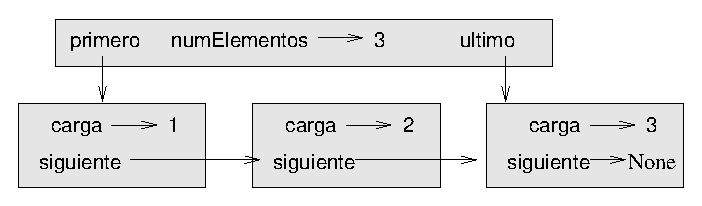
\includegraphics{illustrations/queue1}}
\afterfig

La implementación de \texttt{ColaMejorada} es la siguiente:

\beforeverb 
\begin{pythoncode}
class ColaMejorada:
  def __init__(self):
    self.numElementos = 0
    self.primero   = None
    self.ultimo   = None

  def estaVacia(self):
    return (self.numElementos == 0)
\end{pythoncode}
\afterverb Hasta aquí el único cambio es al nuevo atributo \texttt{ultimo}.
Este debe ser usado en los métodos \texttt{meter} y \texttt{sacar}:

\beforeverb 
\begin{pythoncode}
class ColaMejorada:
  ...
  def meter(self, carga):
    nodo = nodo(carga)
    nodo.siguiente = None
    if self.numElementos == 0:
      # si está vacía, el nuevo nodo es primero y ultimo
      self.primero = self.ultimo = nodo
    else:
      # encontrar el ultimo nodo
      ultimo = self.ultimo
      # pegar el nuevo nodo
      ultimo.siguiente = nodo
      self.ultimo = nodo
    self.numElementos = self.numElementos + 1
\end{pythoncode}
\afterverb Ya que \texttt{ultimo} lleva la pista del último nodo,
no tenemos que buscarlo. Como resultado, este método tiene un tiempo
constante de ejecución.

Hay un precio que pagar por esta mejora. Tenemos que agregar un caso
especial a \texttt{sacar} que asigne a \texttt{ultimo} el valor \texttt{None}
cuando se saca el único elemento:

\beforeverb 
\begin{pythoncode}
class ColaMejorada:
  ...
  def sacar(self):
    carga     = self.primero.carga
    self.primero = self.primero.siguiente
    self.numElementos = self.numElementos - 1
    if self.numElementos == 0:
      self.ultimo = None
    return carga
\end{pythoncode}
\afterverb Esta implementación es más compleja que la inicial y es
más difícil demostrar su corrección. La ventaja es que hemos logrado
el objetivo —\texttt{meter} y \texttt{sacar} son operaciones que se
ejecutan en un tiempo constante.
\begin{quote}
{\em Como ejercicio, escriba una implementación del TAD Cola usando
una lista de Python. Compare el desempeño de esta implementación con
el de la \texttt{ColaMejorada} para un distintos valores de numElementos.} 
\end{quote}

\section{Cola de prioridad}

\index{cola de prioridad!TAD} \index{TAD!cola de prioridad}

El TAD cola de prioridad tiene la misma interfaz que el TAD Cola,
pero su semántica es distinta.
\begin{description}
\item [{texttt{\_\_init\_\_}:}] inicializa una Cola vacía.
\item [{texttt{meter}:}] agrega un objeto a la Cola.
\item [{texttt{sacar}:}] saca y retorna un objeto de la Cola. El objeto
que se retorna es el de la mas alta prioridad.
\item [{texttt{estaVacia}:}] verifica si la Cola está vacía.
\end{description}
La diferencia semántica está en el objeto que se saca, que necesariamente
no es el primero que se agregó. En vez de esto, es el que tiene el
mayor valor de prioridad. Las prioridades y la manera de compararlas
no se especifica en la implementación de la cola de prioridad. Depende
de cuáles objetos estén en la Cola.

Por ejemplo, si los objetos en la Cola tienen nombres, podríamos escogerlos
en orden alfabético. Si son puntajes de bolos iríamos sacando del
más alto al más bajo; pero si son puntajes de golf, iríamos del más
bajo al más alto. En tanto que podamos comparar los objetos en la
Cola, podemos encontrar y sacar el que tenga la prioridad más alta.

Esta implementación de la cola de prioridad tiene como atributo una
lista de Python que contiene los elementos en la Cola.

\beforeverb 
\begin{pythoncode}
class ColaPrioridad:
  def __init__(self):
    self.items = []

  def estaVacia(self):
    return self.items == []

  def meter(self, item):
    self.items.append(item)
\end{pythoncode}
\afterverb El método de inicialización, \texttt{estaVacia}, y \texttt{meter}
solo son barniz para operaciones sobre listas. El único interesante
es \texttt{sacar}:

\beforeverb 
\begin{pythoncode}
class ColaPrioridad:
  ...
  def sacar(self):
    maxi = 0
    for i in range(1,len(self.items)):
      if self.items[i] > self.items[maxi]:
        maxi = i
    item = self.items[maxi]
    self.items[maxi:maxi+1] = []
    return item
\end{pythoncode}
\afterverb Al iniciar cada iteración, \texttt{maxi} almacena el índice
del ítem más grande (con la prioridad más alta) que hayamos encontrado
{\em hasta el momento}. En cada iteración, el programa compara
el \texttt{i}ésimo ítem con el que iba ganando. Si el nuevo es mejor,
el valor de \texttt{maxi} se actualiza con el de \texttt{i}.

\index{recorrido}

Cuando el \texttt{for} se completa, \texttt{maxi} es el índice con
el mayor ítem de todos. Éste se saca de la lista y se retorna.

Probemos la implementación:

\beforeverb 
\begin{pyconcode}
>>> q = ColaPrioridad()
>>> q.meter(11)
>>> q.meter(12)
>>> q.meter(14)
>>> q.meter(13)
>>> while not q.estaVacia(): print(q.sacar())
14
13
12
11
\end{pyconcode}
\afterverb Si la Cola contiene números o cadenas, se sacan en orden
alfabético o numérico, del más alto al más bajo. Python puede encontrar
el mayor entero o cadena a través de los operadores de comparación
primitivos.

Si la Cola contiene otro tipo de objeto, creado por el programador,
tiene que proporcionar el método \texttt{\_\_cmp\_\_}. Cuando \texttt{sacar}
use al operador \texttt{>} para comparar items, estaría llamando el
método \texttt{\_\_cmp\_\_} sobre el primero y pasándole al segundo
como parámetro. En tanto que \texttt{\_\_cmp\_\_} funcione correctamente,
la cola de prioridad será correcta.

\section{La clase \texttt{golfista}}

\index{golfista} \index{clase!golfista} \index{prioridad} \index{sobrecarga de operadores}
\index{sobrecarga!operador}

Un ejemplo poco usado de definición de prioridad es la clase \texttt{golfista}
que lleva el registro de los nombres y los puntajes de jugadores de
golf. Primero definimos \texttt{\_\_init\_\_} y \texttt{\_\_str\_\_}:

\beforeverb 
\begin{pythoncode}
class golfista:
  def __init__(self, nombre, puntaje):
    self.nombre = nombre
    self.puntaje= puntaje

  def __str__(self):
    return "%-16s: %d" % (self.nombre, self.puntaje)
\end{pythoncode}
\afterverb \texttt{\_\_str\_\_} utiliza el operador de formato para
poner los nombres y los puntajes en dos columnas.

\index{operador de formato} \index{operador!de formato}

A continuación definimos una versión de \texttt{\_\_cmp\_\_} en la
que el puntaje mas bajo tenga la prioridad mas alta. Recuerde que
para Python \texttt{\_\_cmp\_\_} retorna 1 si \texttt{self} es ``mayor
que'' \texttt{otro}, -1 si \texttt{self} es ``menor'' otro, y 0
si son iguales.

\beforeverb 
\begin{pythoncode}
class golfista:
  ...
  def __cmp__(self, otro):
    # el menor tiene mayor prioridad
    if self.puntaje < otro.puntaje: return  1   
    if self.puntaje > otro.puntaje: return -1
    return 0
\end{pythoncode}
\afterverb Ahora estamos listos para probar la cola de prioridad
almacenando instancias de la clase \texttt{golfista}:

\beforeverb 
\begin{pyconcode}
>>> tiger = golfista("Tiger Woods",    61)
>>> phil  = golfista("Phil Mickelson", 72)
>>> hal   = golfista("Hal Sutton",     69)
>>>
>>> pq = ColaPrioridad()
>>> pq.meter(tiger)
>>> pq.meter(phil)
>>> pq.meter(hal)
>>> while not pq.estaVacia(): print(pq.sacar())
Tiger Woods    : 61
Hal Sutton     : 69
Phil Mickelson : 72
\end{pyconcode}
\afterverb
\begin{quote}
{\em Como ejercicio, escriba una implementación del TAD cola de
prioridad TAD usando una lista enlazada. Ésta debe mantenerse ordenada,
de forma que sacar sea una operación de tiempo constante. Compare
el desempeño de esta implementación con la implementación basada en
listas de Python.} 
\end{quote}

\section{Glosario}

\index{Cola} \index{política de atención} \index{PEPS} \index{cola de prioridad}
\index{barniz} \index{tiempo constante} \index{tiempo lineal} \index{desempeño}
\index{Cola enlazada} \index{buffer circular} \index{clase abstracta}
\index{interfaz}
\begin{description}
\item [{Cola:}] conjunto ordenado de objetos (o personas) esperando a que
se les preste algún servicio
\item [{Cola:}] TAD con las operaciones que se realizan en una Cola.
\item [{Política de atención:}] reglas que determinan cuál es el siguiente
objeto que se saca (atiende) en una Cola.
\item [{PEPS:}] ``Primero que Entra, Primero que Sale'' , política de
atención en la que se saca el primer elemento de la Cola.
\item [{Atención por prioridad:}] una política de atención en la que
se saca el elemento de la Cola que tenga la mayor prioridad.
\item [{Cola de prioridad:}] un TAD que define las operaciones que se
pueden realizar en una cola de prioridad.
\item [{Cola enlazada:}] implementación de una Cola que utiliza una lista
enlazada.
\item [{Desempeño:}] toda función de un TAD realiza un número de operaciones
básicas que dependen del número de elementos que éste contiene en
un momento dado. Por medio de este número de operaciones básicas se
pueden comparar distintas alternativas de implementación de una operación.
\item [{Tiempo constante:}] desempeño de una operación, cuyo tiempo de
ejecución no depende del tamaño de la estructura de datos.
\item [{Tiempo lineal:}] desempeño de una operación, cuyo tiempo de ejecución
es una función lineal del tamaño de la estructura de datos.
\end{description}

